\chapter{Fundamentação teórica} \label{RevisaoBibliografica}

Este capítulo apresenta os fundamentos teóricos necessários .

\subsection{Tensão e Deformação}

Quando uma carga externa age sobre uma área seccionada de um corpo como na  \ref{pontoesp}, como resultado, aparecem forças internas agindo sobre essa mesma seção. Esse fenômeno é denominado tensão, que representa o quociente de uma força sobre uma área. Quando a força agir sobre a área perpendicularmente, tem-se a tensão normal \(\sigma \). Porém, quando a força agir tangencialmente à área, será denominada como tensão de cisalhamento \(\tau \), \cite{Hibbeler2009}.

\begin{figure}[!htb]
   \centering
     \caption{Cargas sobre um ponto.}
    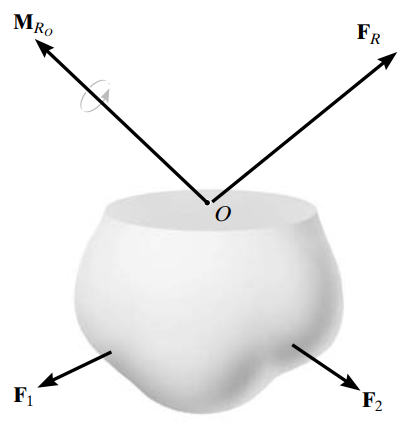
\includegraphics[width=0.3\linewidth]{Figuras/pontoespecifico.png}\\
    \hspace{1.5cm}\raggedright \fontsize{10}{12}\selectfont{Fonte: \textcite{Hibbeler2009}.}
    \label{pontoesp}
\end{figure}

Segundo \textcite{Hibbeler2009}, para um elemento de área infinitesimal \(\Delta \)A, a tensão normal \( \sigma_z \) se dará por um limite da razão da força \( F_z \) com a sua área tendendo a zero, como na equação \ref{eq1}:

\begin{equation}
\label{eq1}
\sigma_z =  \lim_{\Delta A\to0} \frac{\Delta F_z}{\Delta A} 
\end{equation}
\bigskip

Se essa força tracionar o elemento \(\Delta \)A, será denominada tensão de tração, ao passo que se comprimir o elemento, receberá o nome de tensão de compressão.
Para a tensão de cisalhamento (\(\tau \)) ocorre o mesmo fenômeno, dando origem a 2 componentes que agem tangencialmente à área infinitesimal \(\Delta \)A, sendo estes perpendiculares entre si, conforme as equações \ref{eq2a} e \ref{eq2b} \cite{Hibbeler2009}:

\begin{equation}
\label{eq2a}
\tau_{zx} =  \lim_{\Delta A\to0} \frac{\Delta F_x}{\Delta A}
\end{equation}
\bigskip

\begin{equation}
\label{eq2b}
\tau_{zy} =  \lim_{\Delta A\to0} \frac{\Delta F_y}{\Delta A}
\end{equation}
\bigskip

